\documentclass[a4paper]{scrartcl}
\usepackage{amssymb, amsmath} % needed for math
\usepackage{mathtools}      % \xRightarrow
\usepackage[utf8]{inputenc} % this is needed for umlauts
\usepackage[english]{babel} % this is needed for umlauts
\usepackage[T1]{fontenc}    % this is needed for correct output of umlauts in pdf
\usepackage[margin=2.5cm]{geometry} %layout
\usepackage{hyperref}   % links im text
\usepackage{braket}         % needed for \Set
\usepackage{parskip}
\usepackage[colorinlistoftodos]{todonotes}
\usepackage{pgfplots}
\pgfplotsset{compat=1.7,compat/path replacement=1.5.1}
\usepackage{tikz}
\usepackage[framed,amsmath,thmmarks,hyperref]{ntheorem}
\usepackage{framed}
\usepackage{nicefrac}
\usepackage{siunitx}

%%%%%%%%%%%%%%%%%%%%%%%%%%%%%%%%%%%%%%%%%%%%%%%%%%%%%%%%%%%%%%%%%%%%%
% Define theorems                                                   %
%%%%%%%%%%%%%%%%%%%%%%%%%%%%%%%%%%%%%%%%%%%%%%%%%%%%%%%%%%%%%%%%%%%%%
\theoremstyle{break}
\setlength\theoremindent{0.7cm}
\theoremheaderfont{\kern-0.7cm\normalfont\bfseries} 
\theorembodyfont{\normalfont} % nicht mehr kursiv

\def\mdr{\ensuremath{\mathbb{R}}}
\renewcommand{\qed}{\hfill\blacksquare}

\newframedtheorem{theorem}{Theorem}
\newframedtheorem{lemma}[theorem]{Lemma}
\newtheorem{plaindefinition}{Definition}
\newenvironment{definition}{\begin{plaindefinition}}{\end{plaindefinition}}
\newenvironment{definition*}{\begin{plaindefinition*}}{\end{plaindefinition*}}
\newtheorem{example}{Example}
\theoremstyle{nonumberplain}
\newtheorem{proof}{Proof:}
%%%%%%%%%%%%%%%%%%%%%%%%%%%%%%%%%%%%%%%%%%%%%%%%%%%%%%%%%%%%%%%%%%%%%

\title{Minimal distance to a cubic function}
\author{Martin Thoma}

\hypersetup{ 
  pdfauthor   = {Martin Thoma}, 
  pdfkeywords = {}, 
  pdftitle    = {Minimal Distance} 
}

\def\mdr{\ensuremath{\mathbb{R}}}

%%%%%%%%%%%%%%%%%%%%%%%%%%%%%%%%%%%%%%%%%%%%%%%%%%%%%%%%%%%%%%%%%%%%%
% Begin document                                                    %
%%%%%%%%%%%%%%%%%%%%%%%%%%%%%%%%%%%%%%%%%%%%%%%%%%%%%%%%%%%%%%%%%%%%%
\begin{document}
\maketitle
\begin{abstract}
When you want to develop a selfdriving car, you have to plan which path 
it should take. A reasonable choice for the representation of
paths are cubic splines. You also have to be able to calculate
how to steer to get or to remain on a path. A way to do this
is applying the \href{https://en.wikipedia.org/wiki/PID_algorithm}{PID algorithm}.
This algorithm needs to know the signed current error. So you need to 
be able to get the minimal distance of a point to a cubic spline combined with the direction (left or right).
As you need to get the signed error (and one steering direction might
be prefered), it is not only necessary to
get the minimal absolute distance, but might also help to get all points
on the spline with minimal distance.

In this paper I want to discuss how to find all points on a cubic 
function with minimal distance to a given point.
As other representations of paths might be easier to understand and
to implement, I will also cover the problem of finding the minimal
distance of a point to a polynomial of degree 0, 1 and 2.
\end{abstract}

\section{Description of the Problem}
Let $f: \mdr \rightarrow \mdr$ be a polynomial function and $P \in \mdr^2$
be a point. Let $d_{P,f}: \mdr \rightarrow \mdr_0^+$
be the Euklidean distance of a point $P$ and a point $\left (x, f(x) \right )$
on the graph of $f$:
\[d_{P,f} (x) := \sqrt{(x_P - x)^2 + (y_P - f(x))^2}\]

Now there is finite set $M = \Set{x_1, \dots, x_n}$ of minima for given $f$ and $P$:
\[M = \Set{x \in \mdr | d_{P,f}(x) = \min_{\overline{x} \in \mdr} d_{P,f}(\overline{x})}\] 

But minimizing $d_{P,f}$ is the same as minimizing $d_{P,f}^2$:
\begin{align}
    d_{P,f}(x)^2    &= \sqrt{(x_P - x)^2 + (y_P - f(x))^2}^2\\
                &= x_p^2 - 2x_p x + x^2 + y_p^2 - 2y_p f(x) + f(x)^2
\end{align}

\begin{theorem}[Fermat's theorem about stationary points]\label{thm:required-extremum-property}
    Let $x_0$ be a local extremum of a differentiable function $f: \mathbb{R} \rightarrow \mathbb{R}$.

    Then: $f'(x_0) = 0$.
\end{theorem}
\clearpage

%%%%%%%%%%%%%%%%%%%%%%%%%%%%%%%%%%%%%%%%%%%%%%%%%%%%%%%%%%%%%%%%%%%%%
% Constant functions                                                %
%%%%%%%%%%%%%%%%%%%%%%%%%%%%%%%%%%%%%%%%%%%%%%%%%%%%%%%%%%%%%%%%%%%%%
\section{Minimal distance to a constant function}
Let $f(x) = c$ with $c \in \mdr$ be a constant function. 

\begin{figure}[htp]
    \centering
    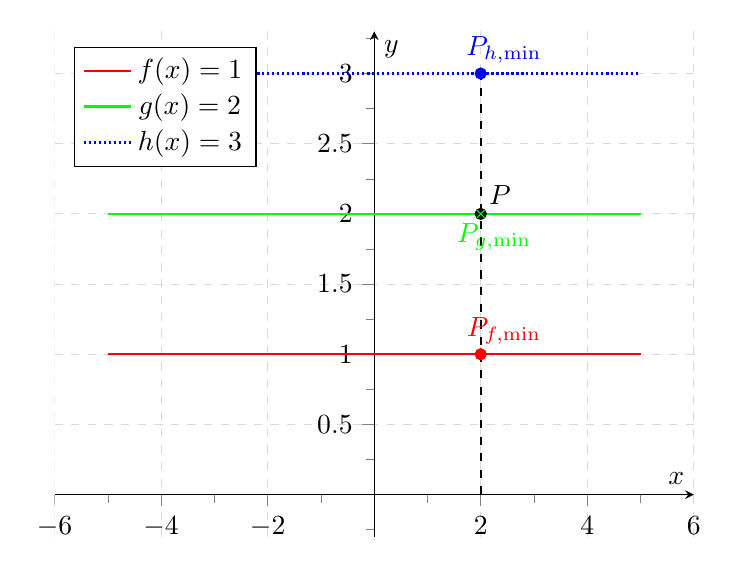
\begin{tikzpicture}
        \begin{axis}[
            legend pos=north west,
            axis x line=middle,
            axis y line=middle,
            grid = major,
            width=0.8\linewidth,
            height=8cm,
            grid style={dashed, gray!30},
            xmin=-5, % start the diagram at this x-coordinate
            xmax= 5, % end   the diagram at this x-coordinate
            ymin= 0, % start the diagram at this y-coordinate
            ymax= 3, % end   the diagram at this y-coordinate
            axis background/.style={fill=white},
            xlabel=$x$,
            ylabel=$y$,
            tick align=outside,
            minor tick num=-3,
            enlargelimits=true,
            tension=0.08]
          \addplot[domain=-5:5, thick,samples=50, red] {1};
          \addplot[domain=-5:5, thick,samples=50, green] {2};
          \addplot[domain=-5:5, thick,samples=50, blue, densely dotted] {3};
          \addplot[black, mark = *, nodes near coords=$P$,every node near coord/.style={anchor=225}] coordinates {(2, 2)};
          \addplot[blue, mark = *, nodes near coords=$P_{h,\text{min}}$,every node near coord/.style={anchor=225}] coordinates {(2, 3)};
          \addplot[green, mark = x, nodes near coords=$P_{g,\text{min}}$,every node near coord/.style={anchor=120}] coordinates {(2, 2)};
          \addplot[red, mark = *, nodes near coords=$P_{f,\text{min}}$,every node near coord/.style={anchor=225}] coordinates {(2, 1)};
          \draw[thick, dashed] (axis cs:2,0) -- (axis cs:2,3);
          \addlegendentry{$f(x)=1$}
          \addlegendentry{$g(x)=2$}
          \addlegendentry{$h(x)=3$}
        \end{axis} 
    \end{tikzpicture}
    \caption{Three constant functions and their points with minimal distance}
    \label{fig:constant-min-distance}
\end{figure}

Then $(x_P,f(x_P))$ has
minimal distance to $P$. Every other point has higher distance.
See Figure~\ref{fig:constant-min-distance}.

%%%%%%%%%%%%%%%%%%%%%%%%%%%%%%%%%%%%%%%%%%%%%%%%%%%%%%%%%%%%%%%%%%%%%
% Linear functions                                                  %
%%%%%%%%%%%%%%%%%%%%%%%%%%%%%%%%%%%%%%%%%%%%%%%%%%%%%%%%%%%%%%%%%%%%%
\section{Minimal distance to a linear function}
Let $f(x) = m \cdot x + t$ with $m \in \mdr \setminus \Set{0}$ and 
$t \in \mdr$ be a linear function.

\begin{figure}[htp]
    \centering
    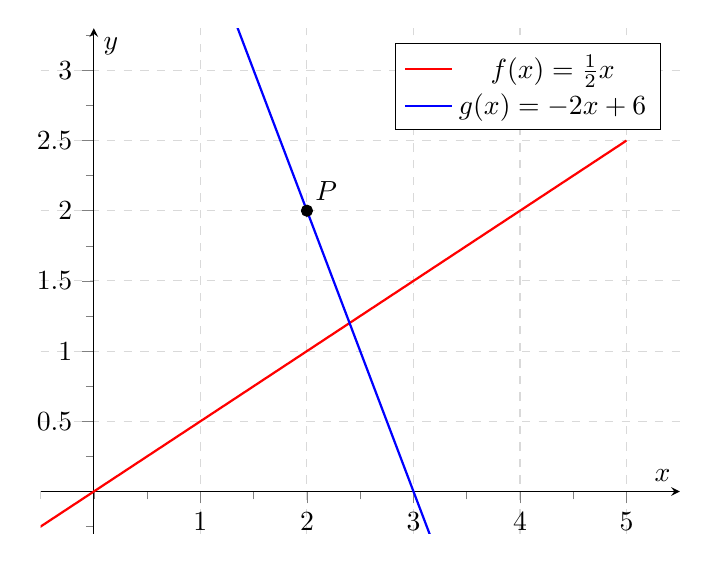
\begin{tikzpicture}
        \begin{axis}[
            legend pos=north east,
            axis x line=middle,
            axis y line=middle,
            grid = major,
            width=0.8\linewidth,
            height=8cm,
            grid style={dashed, gray!30},
            xmin= 0, % start the diagram at this x-coordinate
            xmax= 5, % end   the diagram at this x-coordinate
            ymin= 0, % start the diagram at this y-coordinate
            ymax= 3, % end   the diagram at this y-coordinate
            axis background/.style={fill=white},
            xlabel=$x$,
            ylabel=$y$,
            tick align=outside,
            minor tick num=-3,
            enlargelimits=true,
            tension=0.08]
          \addplot[domain=-5:5, thick,samples=50, red] {0.5*x};
          \addplot[domain=-5:5, thick,samples=50, blue] {-2*x+6};
          \addplot[black, mark = *, nodes near coords=$P$,every node near coord/.style={anchor=225}] coordinates {(2, 2)};
          \addlegendentry{$f(x)=\frac{1}{2}x$}
          \addlegendentry{$g(x)=-2x+6$}
        \end{axis} 
    \end{tikzpicture}
    \caption{The shortest distance of $P$ to $f$ can be calculated by using the perpendicular}
    \label{fig:linear-min-distance}
\end{figure}

Now you can drop a perpendicular $f_\bot$ through $P$ on $f(x)$. The 
slope of $f_\bot$ is $- \frac{1}{m}$ and $t_\bot$ can be calculated:\nobreak
\begin{align}
                 f_\bot(x) &= - \frac{1}{m} \cdot x + t_\bot\\
    \Rightarrow        y_P &= - \frac{1}{m} \cdot x_P + t_\bot\\
    \Leftrightarrow t_\bot &= y_P + \frac{1}{m} \cdot x_P
\end{align}

The point $(x, f(x))$ where the perpendicular $f_\bot$ crosses $f$
is calculated this way:
\begin{align}
    f(x) &= f_\bot(x)\\
    \Leftrightarrow m \cdot x + t &= - \frac{1}{m} \cdot x + \left(y_P + \frac{1}{m} \cdot x_P \right)\\
    \Leftrightarrow \left (m + \frac{1}{m} \right ) \cdot x &= y_P + \frac{1}{m} \cdot x_P - t\\
    \Leftrightarrow x &= \frac{m}{m^2+1} \left ( y_P + \frac{1}{m} \cdot x_P - t \right )
\end{align}

There is only one point with minimal distance. See Figure~\ref{fig:linear-min-distance}.
\clearpage
%%%%%%%%%%%%%%%%%%%%%%%%%%%%%%%%%%%%%%%%%%%%%%%%%%%%%%%%%%%%%%%%%%%%%
% Quadratic functions                                               %
%%%%%%%%%%%%%%%%%%%%%%%%%%%%%%%%%%%%%%%%%%%%%%%%%%%%%%%%%%%%%%%%%%%%%
\section{Minimal distance to a quadratic function}
Let $f(x) = a \cdot x^2 + b \cdot x + c$ with $a \in \mdr \setminus \Set{0}$ and 
$b, c \in \mdr$ be a quadratic function.

\begin{figure}[htp]
    \centering
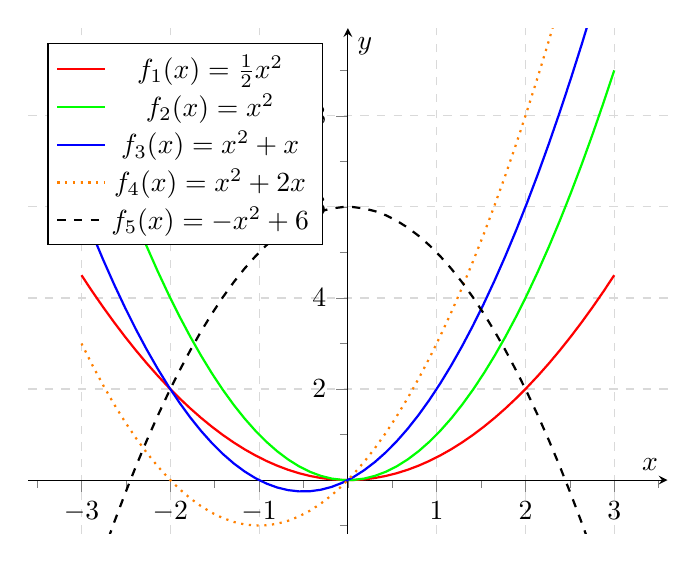
\begin{tikzpicture}
    \begin{axis}[
        legend pos=north west,
        axis x line=middle,
        axis y line=middle,
        grid = major,
        width=0.8\linewidth,
        height=8cm,
        grid style={dashed, gray!30},
        xmin=-3,    % start the diagram at this x-coordinate
        xmax= 3,    % end   the diagram at this x-coordinate
        ymin=-0.25, % start the diagram at this y-coordinate
        ymax= 9,    % end   the diagram at this y-coordinate
        axis background/.style={fill=white},
        xlabel=$x$,
        ylabel=$y$,
        tick align=outside,
        minor tick num=-3,
        enlargelimits=true,
        tension=0.08]
      \addplot[domain=-3:3, thick,samples=50, red]    {0.5*x*x}; 
      \addplot[domain=-3:3, thick,samples=50, green]  { x*x}; 
      \addplot[domain=-3:3, thick,samples=50, blue]   { x*x +   x};
      \addplot[domain=-3:3, thick,samples=50, orange,dotted] { x*x + 2*x};
      \addplot[domain=-3:3, thick,samples=50, black,dashed]  {-x*x + 6};
      \addlegendentry{$f_1(x)=\frac{1}{2}x^2$}
      \addlegendentry{$f_2(x)=x^2$}
      \addlegendentry{$f_3(x)=x^2+x$}
      \addlegendentry{$f_4(x)=x^2+2x$}
      \addlegendentry{$f_5(x)=-x^2+6$}
    \end{axis} 
\end{tikzpicture}
    \caption{Quadratic functions}
\end{figure}

\subsection{Calculate points with minimal distance}
In this case, $d_{P,f}^2$ is polynomial of degree 4. 
We use Theorem~\ref{thm:required-extremum-property}:\nobreak
\begin{align}
    0     &\overset{!}{=} (d_{P,f}^2)'\\
          &= -2 x_p + 2x -2y_p f'(x) + \left (f(x)^2 \right )'\\
          &= -2 x_p + 2x -2y_p f'(x) + 2 f(x) \cdot f'(x) \rlap{\hspace*{3em}(chain rule)}\label{eq:minimizingFirstDerivative}\\
\Leftrightarrow 0 &\overset{!}{=} -x_p + x -y_p f'(x) + f(x) \cdot f'(x) \rlap{\hspace*{3em}(divide by 2)}\label{eq:minimizingFirstDerivative}\\
          &= -x_p + x -y_p (2ax+b) + (ax^2+bx+c)(2ax+b)\\
          &= -x_p + x -y_p \cdot 2ax- y_p b + (2 a^2 x^3+2 a b x^2+2 a c x+ab x^2+b^2 x+bc)\\
          &= -x_p + x -2y_p ax- y_p b + (2a^2 x^3 + 3 ab x^2 + 2acx + b^2 x + bc)\\
          &= 2a^2 x^3 + 3 ab x^2 + (1 -2y_p a+ 2ac + b^2)x +(bc-by_p-x_p)\label{eq:quadratic-derivative-eq-0}
\end{align}

This is an algebraic equation of degree 3.
There can be up to 3 solutions in such an equation. Those solutions
can be found with a closed formula.

\todo[inline]{Where are those closed formulas?}

\begin{example}
    Let $a = 1,  b = 0,  c= 1, x_p= 0, y_p = 1$.
    So $f(x) = x^2 + 1$ and $P(0, 1)$.

\begin{align}
    0 &\stackrel{!}{=} 4 x^3 - 2x\\
      &=2x(2x^2 - 1)\\
    \Rightarrow x_1 &= 0 \;\;\; x_{2,3} = \pm \frac{1}{\sqrt{2}}
\end{align}

As you can easily verify, only $x_1$ is a minimum of $d_{P,f}$.
\end{example}


\subsection{Number of points with minimal distance}
\begin{theorem}
    A point $P$ has either one or two points on the graph of a 
    quadratic function $f$ that are closest to $P$.
\end{theorem}

In the following, I will do some transformations with $f = f_0$ and
$P = P_0$ .

Moving $f_0$ and $P_0$ simultaneously in $x$ or $y$ direction does 
not change the minimum distance. Furthermore, we can find the 
points with minimum distance on the moved situation and calculate
the minimum points in the original situation.

First of all, we move $f_0$ and $P_0$ by $\frac{b}{2a}$ in $x$ direction, so
\[f_1(x) = ax^2 - \frac{b^2}{4a} + c \;\;\;\text{ and }\;\;\; P_1 = \left (x_p+\frac{b}{2a},\;\; y_p \right )\]

Because:\footnote{The idea why you subtract $\frac{b}{2a}$ within
$f$ is that when you subtract something from $x$ before applying
$f$ it takes more time ($x$ needs to be bigger) to get to the same
situation. So to move the whole graph by $1$ to the left whe have
to add $+1$.}
\begin{align}
    f(x-\nicefrac{b}{2a}) &= a (x-\nicefrac{b}{2a})^2 + b (x-\nicefrac{b}{2a}) + c\\
    &= a (x^2 - \nicefrac{b}{a} x + \nicefrac{b^2}{4a^2}) + bx - \nicefrac{b^2}{2a} + c\\
    &= ax^2 - bx + \nicefrac{b^2}{4a} + bx - \nicefrac{b^2}{2a} + c\\
    &= ax^2 -\nicefrac{b^2}{4a} + c
\end{align}


Then move $f_1$ and $P_1$ by $\frac{b^2}{4a}-c$ in $y$ direction. You get:
\[f_2(x) = ax^2\;\;\;\text{ and }\;\;\; P_2 = \Big (\underbrace{x_P+\frac{b}{2a}}_{=: z},\;\; \underbrace{y_P+\frac{b^2}{4a}-c}_{=: w} \Big )\]

\textbf{Case 1:} As $f_2(x) = ax^2$ is symmetric to the $y$ axis, only points 
$P = (0, w)$ could possilby have three minima.

Then compute:
\begin{align}
  d_{P,{f_2}}(x)  &= \sqrt{(x-0)^2 + (f_2(x)-w)^2}\\
    &= \sqrt{x^2 + (ax^2-w)^2}\\
    &= \sqrt{x^2 + a^2 x^4-2aw x^2+w^2}\\
    &= \sqrt{a^2 x^4 + (1-2aw) x^2 + w^2}\\
    &= \sqrt{\left (a^2 x^2 + \frac{1-2 a w}{2} \right )^2 + w^2 - (1-2 a w)^2}\\
    &= \sqrt{\left (a^2 x^2 + \nicefrac{1}{2}-a w \right )^2 + \big (w^2 - (1-2 a w)^2 \big)}
\end{align}

The term 
\[a^2 x^2 + (\nicefrac{1}{2}-a w)\]
should get as close to $0$ as possilbe when we want to minimize 
$d_{P,{f_2}}$. For $w \leq \nicefrac{1}{2a}$ you only have $x = 0$ as a minimum.
For all other points $P = (0, w)$, there are exactly two minima $x_{1,2} = \pm \sqrt{aw - \nicefrac{1}{2}}$.

\textbf{Case 2:} $P = (z, w)$ is not on the symmetry axis, so $z \neq 0$. Then you compute:
\begin{align}
  d_{P,{f_2}}(x)  &= \sqrt{(x-z)^2 + (f(x)-w)^2}\\
    &= \sqrt{(x^2 - 2zx + z^2) + ((ax^2)^2 - 2 awx^2 + w^2)}\\
    &= \sqrt{a^2x^4 + (1- 2 aw)x^2 +(- 2z)x + z^2 + w^2}\\
  0 &\stackrel{!}{=} \Big(\big(d_{P, {f_2}}(x)\big)^2\Big)' \\
    &= 4a^2x^3 + 2(1- 2 aw)x +(- 2z)\\
    &= 2 \left (2a^2x^2 + (1- 2 aw) \right )x - 2z\\
    \Leftrightarrow 0 &\stackrel{!}{=} (2a^2x^2  + (1- 2 aw)) x - z\\
    &= 2 a^2 x^3 + (1- 2 aw) x - z\\
\Leftrightarrow 0 &\stackrel{!}{=} x^3 + \underbrace{\frac{(1- 2 aw)}{2 a^2}}_{=: \alpha} x  + \underbrace{\frac{-z}{2 a^2}}_{=: \beta}\\
    &= x^3 + \alpha x + \beta\label{eq:simple-cubic-equation-for-quadratic-distance}
\end{align}

The solution of Equation~\ref{eq:simple-cubic-equation-for-quadratic-distance}
is
\[t := \sqrt[3]{\sqrt{3 \cdot (4a^3 + 27 b^2)} -9b}\]
\[x = \frac{t}{\sqrt[3]{18}} - \frac{\sqrt[3]{\frac{2}{3}} a }{t}\]

\todo[inline]{verify this solution}


\goodbreak
So the solution is given by
\begin{align*}
x_S &:= - \frac{b}{2a} \;\;\;\;\; \text{(the symmetry axis)}\\
\underset{x\in\mdr}{\arg \min d_{P,f}(x)} &= \begin{cases}
     x_1 = +\sqrt{a (y_p + \frac{b^2}{4a} - c) - \frac{1}{2}} + x_S \text{ and }   &\text{if } x_P = x_S \text{ and } y_p + \frac{b^2}{4a} - c >  \frac{1}{2a} \\
     x_2 = -\sqrt{a (y_p + \frac{b^2}{4a} - c) - \frac{1}{2}} + x_S\\
     x_1 = x_S   &\text{if } x_P = x_S \text{ and } y_p + \frac{b^2}{4a} - c \leq  \frac{1}{2a} \\
     x_1 = todo   &\text{if } x_P \neq x_S
    \end{cases}
\end{align*}

\clearpage
%%%%%%%%%%%%%%%%%%%%%%%%%%%%%%%%%%%%%%%%%%%%%%%%%%%%%%%%%%%%%%%%%%%%%
% Cubic                                                             %
%%%%%%%%%%%%%%%%%%%%%%%%%%%%%%%%%%%%%%%%%%%%%%%%%%%%%%%%%%%%%%%%%%%%%
\section{Minimal distance to a cubic function}
Let $f(x) = a \cdot x^3 + b \cdot x^2 + c \cdot x + d$ be a cubic function
with $a \in \mdr \setminus \Set{0}$ and 
$b, c, d \in \mdr$ be a function.

\begin{figure}[htp]
    \centering
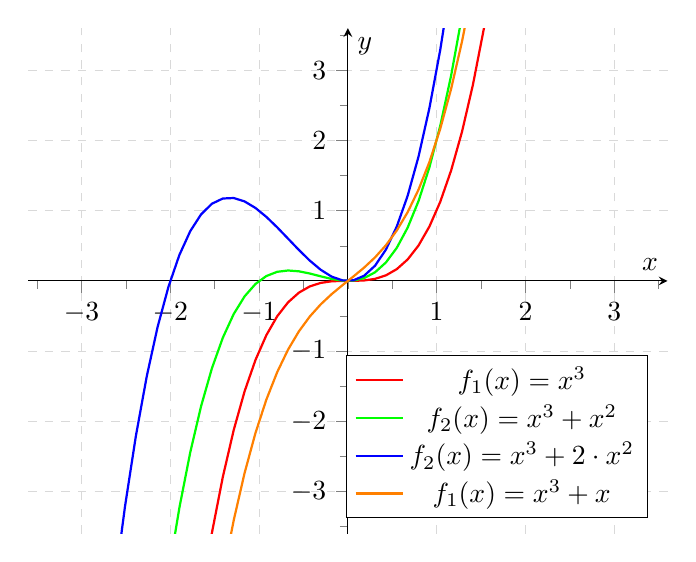
\begin{tikzpicture}
    \begin{axis}[
        legend pos=south east,
        axis x line=middle,
        axis y line=middle,
        grid = major,
        width=0.8\linewidth,
        height=8cm,
        grid style={dashed, gray!30},
        xmin=-3, % start the diagram at this x-coordinate
        xmax= 3, % end   the diagram at this x-coordinate
        ymin=-3, % start the diagram at this y-coordinate
        ymax= 3, % end   the diagram at this y-coordinate
        axis background/.style={fill=white},
        xlabel=$x$,
        ylabel=$y$,
        tick align=outside,
        minor tick num=-3,
        enlargelimits=true,
        tension=0.08]
      \addplot[domain=-3:3, thick,samples=50, red] {x*x*x}; 
      \addplot[domain=-3:3, thick,samples=50, green] {x*x*x+x*x};
      \addplot[domain=-3:3, thick,samples=50, blue] {x*x*x+2*x*x};
      \addplot[domain=-3:3, thick,samples=50, orange] {x*x*x+x}; 
      \addlegendentry{$f_1(x)=x^3$}
      \addlegendentry{$f_2(x)=x^3 + x^2$}
      \addlegendentry{$f_2(x)=x^3 + 2 \cdot x^2$}
      \addlegendentry{$f_1(x)=x^3 + x$}
    \end{axis} 
\end{tikzpicture}
    \caption{Cubic functions}
\end{figure}

%
%\subsection{Special points}
%\todo[inline]{Write this}
%
%\subsection{Voronoi}
%
%For $b^2 \geq 3ac$
%
%\todo[inline]{Write this}

\subsection{Calculate points with minimal distance}
\begin{theorem}
    There cannot be an algebraic solution to the problem of finding 
    a closest point $(x, f(x))$ to a given point $P$ when $f$ is
    a polynomial function of degree $3$ or higher.
\end{theorem}

\begin{proof}
Let $g : \mdr \rightarrow \mdr$ be a polynomial of degree 5
\[g(x) = \tilde{a} x^5 + \tilde{b} x^4 + \tilde{c} x^3 + \tilde{d} x^2 + \tilde{e} x + \tilde{f}\]
with $\tilde{a} \in \mdr_{> 0},\; \tilde{b} \in \mdr \setminus \Set{0}$ and $\tilde{c}, \tilde{d}, \tilde{e}, \tilde{f} \in \mdr$.
Then, according to the Abel-Ruffini theorem, the equation
\[g(x) = 0\]
cannot be solved algebraicly.

%But lets define $a := \frac{\sqrt{\tilde{a}}}{3}$, $b := \frac{\tilde{b}}{5a}$,
%$c : = \frac{\frac{\tilde{c}}{2} - b^2}{2a}$, $d := \frac{\tilde{d}}{3} - bc + $

So you can find $a, b, c, d, x_p, y_p$ such that

\begin{align}
    g(x) &= \underbrace{3 a^2}_{= \tilde{a}} x^5 + \underbrace{5ab}_{= \tilde{b}}x^4 + \underbrace{2(2ac + b^2 )}_{= \tilde{c}}x^3 &+& \underbrace{3(ad+bc-ay_p)}_{= \tilde{d}} x^2 \\
    & &+& \underbrace{(2 b d+c^2+1-2 b y_p)}_{= \tilde{e}}x+\underbrace{c d-c y_p-x_p}_{= \tilde{f}}\\
    &= f'(x) \cdot \left (f(x) - y_p \right ) + (x - x_p)\\
    &= f(x) \cdot f'(x) - y_p f'(x) + x - x_p
\end{align}

And
\begin{align}
  g(x) &\stackrel{!}{=}0\\
\Leftrightarrow 0 &\stackrel{!}{=} 2 f(x) \cdot f'(x) - 2 y_p f'(x) + 2x - 2 x_p\\
    &= -2 x_p + 2x -2y_p(f(x))' + (f(x)^2)'\\
    &= \left ((x-x_p)^2 \right )' + \left ( (f(x) - y_p)^2 \right )'\\
    &= \left ((x-x_p)^2 + (f(x) - y_p)^2 \right )'\\
    &= (d_{P,f}(x)^2)'
\end{align}

    So the problem of finding a closest point $(x, f(x))$ on a 
    cubic function $f$ to $P$ is essentially the same as finding 
    a root of a polynomial function of degree 5. As this cannot
    be solved algebraicly, the problem of finding such a point
    can also not be solved algebraicly.$\qed$
\end{proof}

\todo[inline]{Start with theorem that this problem is not solvable
with analytics only. Use a general 5th degree function and show
that it can be mapped to a $f$ and $P$ instance.}

When you want to calculate points with minimal distance, you can 
take the same approach as in Equation \ref{eq:minimizingFirstDerivative}:

\begin{align}
    0  &\stackrel{!}{=} -2 x_p + 2x -2y_p(f(x))' + (f(x)^2)'\\
       &= 2 f(x) \cdot f'(x) - 2 y_p f'(x) + 2x - 2 x_p\\
       &= f(x) \cdot f'(x) - y_p f'(x) + x - x_p\\
       &= \underbrace{f'(x) \cdot \left (f(x) - y_p \right )}_{\text{Polynomial of degree 5}} + x - x_p
\end{align}

General algebraic equations of degree 5 don't have a solution formula.\footnote{TODO: Quelle}
Although here seems to be more structure, the resulting algebraic
equation can be almost any polynomial of degree 5:\footnote{Thanks to Peter Košinár on \href{http://math.stackexchange.com/a/584814/6876}{math.stackexchange.com} for this one}

\begin{align}
    0  &\stackrel{!}{=} f'(x) \cdot \left (f(x) - y_p \right ) + (x - x_p)\\
    &= \underbrace{3 a^2}_{= \tilde{a}} x^5 + \underbrace{5ab}_{\tilde{b}}x^4 + \underbrace{2(2ac + b^2 )}_{=: \tilde{c}}x^3 &+& \underbrace{3(ad+bc-ay_p)}_{\tilde{d}} x^2 \\
    & &+& \underbrace{(2 b d+c^2+1-2 b y_p)}_{=: \tilde{e}}x+\underbrace{c d-c y_p-x_p}_{=: \tilde{f}}\\
    0 &\stackrel{!}{=} \tilde{a}x^5 + \tilde{b}x^4 + \tilde{c}x^3 + \tilde{d}x^2 + \tilde{e}x + \tilde{f}
\end{align}

\begin{enumerate}
    \item With $a$, we can get any value of $\tilde{a} \in \mdr \setminus \Set{0}$.
    \item With $b$, we can get any value of $\tilde{b} \in \mdr \setminus \Set{0}$.
    \item With $c$, we can get any value of $\tilde{c} \in \mdr$.
    \item With $d$, we can get any value of $\tilde{d} \in \mdr$.
    \item With $y_p$, we can get any value of $\tilde{e} \in \mdr$.
    \item With $x_p$, we can get any value of $\tilde{f} \in \mdr$.
\end{enumerate}

The first restriction only guaratees that we have a polynomial of 
degree 5. The second one is necessary, to get a high range of
$\tilde{e}$.

This means, that there is no solution formula for the problem of 
finding the closest points on a cubic function to a given point.

\subsection{Another approach}
Just like we moved the function $f$ and the point to get in a 
nicer situation, we can apply this approach for cubic functions.

\begin{figure}[htp]
    \centering
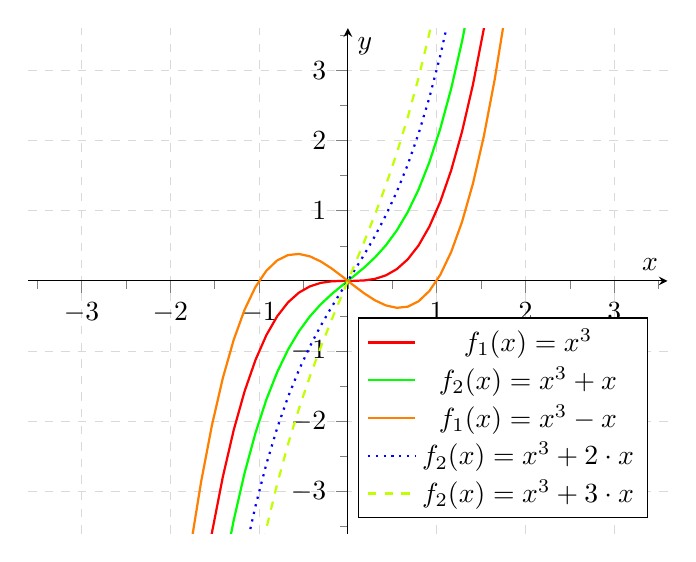
\begin{tikzpicture}
    \begin{axis}[
        legend pos=south east,
        axis x line=middle,
        axis y line=middle,
        grid = major,
        width=0.8\linewidth,
        height=8cm,
        grid style={dashed, gray!30},
        xmin=-3, % start the diagram at this x-coordinate
        xmax= 3, % end   the diagram at this x-coordinate
        ymin=-3, % start the diagram at this y-coordinate
        ymax= 3, % end   the diagram at this y-coordinate
        axis background/.style={fill=white},
        xlabel=$x$,
        ylabel=$y$,
        tick align=outside,
        minor tick num=-3,
        enlargelimits=true,
        tension=0.08]
      \addplot[domain=-3:3, thick,samples=50, red] {x*x*x}; 
      \addplot[domain=-3:3, thick,samples=50, green] {x*x*x+x};
      \addplot[domain=-3:3, thick,samples=50, orange] {x*x*x-x}; 
      \addplot[domain=-3:3, thick,samples=50, blue, dotted] {x*x*x+2*x};
      \addplot[domain=-3:3, thick,samples=50, lime, dashed] {x*x*x+3*x};
      \addlegendentry{$f_1(x)=x^3$}
      \addlegendentry{$f_2(x)=x^3 + x$}
      \addlegendentry{$f_1(x)=x^3 - x$}
      \addlegendentry{$f_2(x)=x^3 + 2 \cdot x$}
      \addlegendentry{$f_2(x)=x^3 + 3 \cdot x$}
    \end{axis} 
\end{tikzpicture}
    \caption{Cubic functions with $b = d = 0$}
\end{figure}

First, we move $f_0$ by $\frac{b}{3a}$ to the right, so

\[f_1(x) = ax^3 + \frac{b^2 (c-1)}{3a} x + \frac{2b^3}{27 a^2} - \frac{bc}{3a} + d \;\;\;\text{ and }\;\;\;P_1 = (x_P + \frac{b}{3a}, y_P)\]

because

\begin{align}
    f_1(x) &= a \left (x - \frac{b}{3a} \right )^3 + b \left (x-\frac{b}{3a} \right )^2 + c \left (x-\frac{b}{3a} \right ) + d\\
           &= a \left (x^3 - 3 \frac{b}{3a}x^2 + 3 (\frac{b}{3a})^2 x - \frac{b^3}{27a^3} \right )
             +b \left (x^2 - \frac{2b}{3a} x + \frac{b^2}{9a^2} \right )
             +c x - \frac{bc}{3a} + d\\
            &= ax^3 - bx^2 + \frac{b^2}{3a}x - \frac{b^3}{27 a^2}\\
            & \;\;\;\;\;\;+ bx^2 - \frac{2b^2}{3a}x + \frac{b^3}{9a^2}\\
            & \;\;\;\;\;\;\;\;\;\;\;\; + c x - \frac{bc}{3a} + d\\
            &= ax^3 + \frac{b^2}{3a}\left (1-2+c \right )x + \frac{b^3}{9a^2} \left (1-\frac{1}{3} \right )- \frac{bc}{3a} + d
\end{align}

\todo[inline]{Which way to move might be clever?}

\subsection{Number of points with minimal distance}
As there is an algebraic equation of degree 5, there cannot be more
than 5 solutions.
\todo[inline]{Can there be 3, 4 or even 5 solutions? Examples!

After looking at function graphs of cubic functions, I'm pretty 
sure that there cannot be 4 or 5 solutions, no matter how you 
chose the cubic function $f$ and $P$.

I'm also pretty sure that there is no polynomial (no matter what degree)
that has more than 3 solutions.}

\section{Newtons method}
\todo[inline]{When does Newtons method converge? How fast?
How to choose starting point?}

\section{Quadratic minimization}
\todo[inline]{TODO}

\section{Conclusion}
\todo[inline]{TODO}

\end{document}
